\documentclass[11pt]{article}
%Gummi|065|=)

\usepackage{array}
\usepackage{graphicx}
\usepackage{tgschola}

\title{\textbf{SSU : Assignment 1} \\ \textbf{SVM detector of generated domain names}}
\author{\textbf{Teymur Azayev}}
\date{}


\begin{document}

\maketitle

\section{Overview}

This document is a short report for the first assignment from the subject. It includes an overview of the task,
how it was solved and the results.

\section{Task}
The task is to create a Kernel SVM classifier to classify strings of DNS addresses to target concept class of
$y \in \{-1,1\}$ where $ -1 $ denotes an address of a legitimate website and the label of $1$ denotes a malicious address which was generated by an algorithm of which we assume to know nothing about. 
\\
To use the strings as input features we first transform them into a String Sub-sequence Kernel (SSK), the definition and methodology of which is described in the task itself. For this task we are given the option of using 
precomputed kernels of size $(m,1000)$ where $m$ is the size of the individual datasets (training, evaluation, test). The task is to learn the SVM classifier on these kernels, as well as the optimal regularization constant
for the classifier out of a given set. 

\section{Implementation}
The task is implemented in Python 2.7. As mentioned, we will make use of the provided pre-computed kernels for all the datasets. We learn an SVM classifier from the library of scikit-learn which uses a lib-svm backend. Other required libraries to run the code are Numpy and Matplotlib. \\
For every regularization constant $c$ we fit the classifier with the training kernels and obtain the amount of support vectors and the training/validation errors so that we can then choose the constant $c$ which resulted in the highest validation error. \\
The whole script runs in less than 2 seconds.

\section{Results}
Below is a table of the support vectors and training/validation errors for various regularization constants.

\begin{center}
\begin{tabular}{ | m{2em} | m{2cm} | m{2cm} | m{2cm} |} 
\hline
C  & Trn error & Eval error & nSV \\ 
\hline
0.01  & 0.245 & 0.256 & [500,500] \\
\hline
0.1  & 0.132 & 0.144 & [437,439] \\
\hline
1  & 0.038 & 0.068 & [265,279] \\
\hline
10  & 0.002 & 0.106 & [202,184] \\
\hline
100  & 0.0 & 0.114 & [199,177] \\


\hline
\end{tabular}
\end{center}

\begin{center}
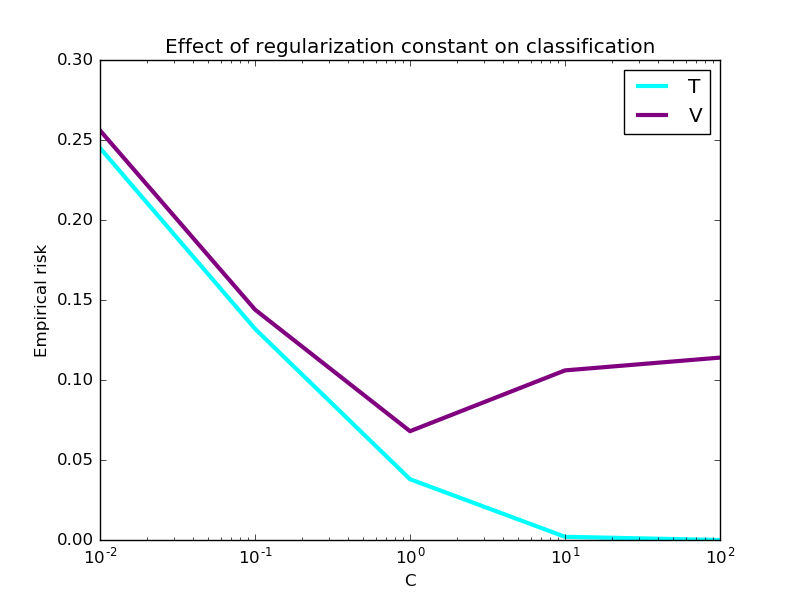
\includegraphics[width=10cm]{/home/shagas/Data/CVUT/SASU/hw_1/Repot/svmoutput.png}
\end{center}

We see on the graph the typical training and evaluation curves. The training error decreases to zero as we increase the $c$ constant and the validation error decreases up to a point where the model starts to overfit. We take this knee point as the best complexity of the model.
The best regularization constant of $c = 1$ is chosen and results in a test error of $0.0785$.

The theoretical minimal value of $\epsilon$ such that the true classification error is in the
interval $(R_{Sl}(h) - \epsilon, R_{Sl} (h) +  \epsilon)$ with the probability $99\%$ at least can be calculated using the Hoeffding inequality. 


\begin{eqnarray}
 \Pr{(\left| \frac{1}{l} \sum\limits_{i=1}^l z^i - \mu  \right| \geq \epsilon) } &\leq& 2e^{-\frac{2l \epsilon^2}{(b-a)^2}}      \nonumber \\
 0.99 &\leq& 2e^{-\frac{2l \epsilon^2}{(b-a)^2}}      \nonumber \\
 \epsilon &\leq& \sqrt{\frac{-(b-a)^2}{2l}\log{\frac{0.99}{2}}}     \nonumber \\
  \epsilon &\leq& 0.0265    \nonumber \\
\end{eqnarray}

\section{Conclusion}
This concludes the report on this task.


\end{document}
